%%%%%%%%%%%%%%%%%%%%%%%%%%%%%%%%%%%%%%%%%
% University/School Laboratory Report
% LaTeX Template
% Version 3.1 (25/3/14)
%
% This template has been downloaded from:
% http://www.LaTeXTemplates.com
%
% Original author:
% Linux and Unix Users Group at Virginia Tech Wiki 
% (https://vtluug.org/wiki/Example_LaTeX_chem_lab_report)
%
% License:
% CC BY-NC-SA 3.0 (http://creativecommons.org/licenses/by-nc-sa/3.0/)
%
%%%%%%%%%%%%%%%%%%%%%%%%%%%%%%%%%%%%%%%%%

%----------------------------------------------------------------------------------------
%	PACKAGES AND DOCUMENT CONFIGURATIONS
%----------------------------------------------------------------------------------------

\documentclass{ctexart}

\usepackage[version=3]{mhchem} % Package for chemical equation typesetting
\usepackage{siunitx} % Provides the \SI{}{} and \si{} command for typesetting SI units
\usepackage{graphicx} % Required for the inclusion of images
\usepackage{natbib} % Required to change bibliography style to APA
\usepackage{amsmath} % Required for some math elements 
%\usepackage{showframe} % for showing page frames


\setlength\parindent{0pt} % Removes all indentation from paragraphs

\renewcommand{\labelenumi}{\alph{enumi}.} % Make numbering in the enumerate environment by letter rather than number (e.g. section 6)

%\usepackage{times} % Uncomment to use the Times New Roman font

%==========pesusdo codes
\usepackage[linesnumbered,boxed]{algorithm2e}
%\renewcommand{\algorithmcfname}{算法}
\renewcommand{\repeat}{Repeat}

%==========citation===========
%\usepackage{cite}
\usepackage{url}


% ==========添加首行缩进,两个字符===========
\usepackage{indentfirst}
\setlength{\parindent}{2em}
% ==========强制图片位置===========
\usepackage{float}

%----------------------------------------------------------------------------------------
%	DOCUMENT INFORMATION
%----------------------------------------------------------------------------------------

\title{逻辑回归} % Title

%\author{fengmi \textsc{Feng}} % Author name

\author{Mia Feng} % Author name

\date{\today} % Date for the report

\begin{document}

\maketitle % Insert the title, author and date

%\begin{center}
%\begin{tabular}{l r}
%Date Performed: & January 1, 2012 \\ % Date the experiment was performed
%Partners: & James Smith \\ % Partner names
%& Mary Smith \\
%Instructor: & Professor Smith % Instructor/supervisor
%\end{tabular}
%\end{center}

% If you wish to include an abstract, uncomment the lines below
% \begin{abstract}
% Abstract text
% \end{abstract}

%----------------------------------------------------------------------------------------
%	SECTION 1
%----------------------------------------------------------------------------------------

\section{概述}
逻辑回归是广义线性模型的一种,适用的数据为可分的。主要用于解决二分类问题,也可以扩展至多分类问题
%To determine the atomic weight of magnesium via its reaction with oxygen and to study the stoichiometry of the reaction (as defined in \ref{definitions}):
求解目标:分类超平面,以二维空间为例,求解一条直线
\begin{equation}
y = b+\theta_1x_1+\theta_2x_2=\theta^{\mathbf{T}}x+b
\end{equation}
求解思路:求解$\theta$的控制方程选择概率描述。使样本点被分类至真实标签的概率最大。推导证明logistic分布的鲁棒性最好,(见LogisticRegressionMaxEnt.pdf)简单来说,因为$p\big(y|x\big)\sim Bernoulli$,根据最大熵原则求解分布(也就是说这个分布应该在满足假设的前提下越均匀越好),推导得到线性模型
$f\big( \theta x \big)$,结果为sigmoid函数,即Bernoulli的指数家族形式

求解方法:最大似然估计

迭代方法:gradient ascent


% If you have more than one objective, uncomment the below:
%\begin{description}
%\item[First Objective] \hfill \\
%Objective 1 text
%\item[Second Objective] \hfill \\
%Objective 2 text
%\end{description}

\subsection{推导}
\label{derivations}
\begin{description}
\item[Sigmoid函数]
\begin{equation}
h_\theta\big(x\big) =\frac{1}{1+e^{-\theta^{\mathbf{T}}x}}
\end{equation}
基于二分类的假定,每个样本点的概率为
\begin{equation}
p\big(y|x,\theta \big) = {h_\theta\big(x\big)}^y{\big(1-h_\theta\big(x\big)\big)}^{1-y}
\end{equation}
这里只是一个技巧性的推导,代入标签值计算一下即可得到。

又基于i.i.d.假设(独立同分布),$m$个样本点的后验概率为:
\begin{equation}
L\big(\theta\big)=\prod_{i=1}^{m}p\big(y_i|x_i,\theta \big) =\prod_{i=1}^{m} {h_\theta\big(x_i\big)}^y_i{\big(1-h_\theta\big(x_i\big)\big)}^{1-y_i}
\end{equation}
为便于计算,取对数
\begin{equation}
L\big(\theta\big)=\ln L\big(\theta\big)=\sum_{i=1}^{m} y_i\ln {h_\theta\big(x_i\big)}+\big(1-y_i\big) \ln {\big(1-h_\theta\big(x_i\big)\big)}
\end{equation}
接下来计算梯度,设置梯度更新,迭代求解$\theta$
参考的blog,打字太多不写了,把他\cite{lr:implement}的推导粘过来了,推倒还是很明了的。梯度:
\begin{figure}[H]
\begin{center}
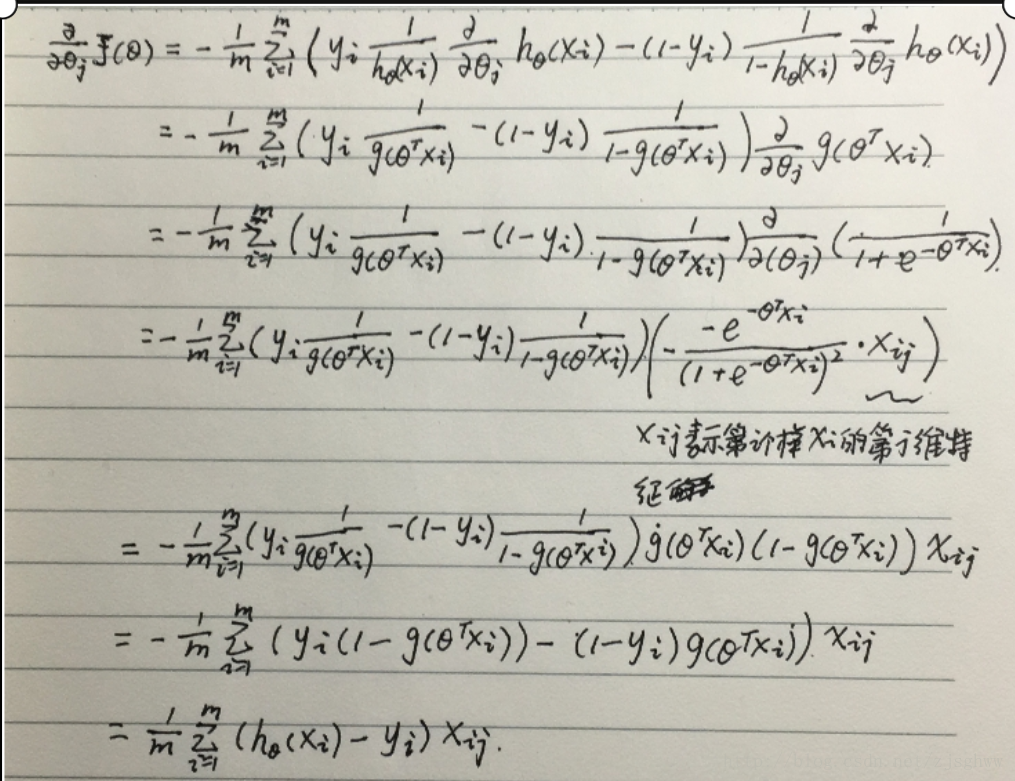
\includegraphics[width=0.8\textwidth]{partialDerivations} % Include the image placeholder.png
\caption{Partial gradient derivation}
\end{center}
\end{figure}

梯度更新公式:
\begin{equation}
\theta_j^{t+1}=\theta_j^t+\alpha\frac{\partial}{\partial \theta_j}L\big(\theta_j\big)=\theta_j^t+\alpha\frac{1}{m}\sum_{i=1}^{m}\big(h_\theta\big(x_i\big)-y_i\big)x_{ij}
\end{equation}

%\item[Atomic mass]
%The mass of an atom of a chemical element expressed in atomic mass units. It is approximately equivalent to the number of protons and neutrons in the atom (the mass number) or to the average number allowing for the relative abundances of different isotopes. 
\end{description} 

 
%----------------------------------------------------------------------------------------
%	SECTION 2
%----------------------------------------------------------------------------------------

\section{Pesudo Code}

\begin{tabular}{ll}
1. 初始化回归系数$\theta$\\
2.重复下面步骤直至收敛\\
\quad$ \left\{ \right.$ \\
\quad \quad 计算整个数据集的梯度\\
\quad \quad 使用公式$\big(6\big)$更新梯度\\
\quad $\left. \right\}$ \\
3.返回回归系数$\theta$

\end{tabular}
\\
\\
Note:程序实现中gradient ascent和gradient descent都是可以的,全看损失函数怎么写。如果计算的是$h\big(x\big)-y$,那么用gradient descent;反之如果计算的是$y-h\big(x\big)$,那么用gradient ascent。
%----------------------------------------------------------------------------------------
%	SECTION 3
%----------------------------------------------------------------------------------------
%

%\section{Sample Calculation}
%
%\begin{tabular}{ll}
%Mass of magnesium metal & = \SI{8.59}{\gram} - \SI{7.28}{\gram}\\
%& = \SI{1.31}{\gram}\\
%Mass of magnesium oxide & = \SI{9.46}{\gram} - \SI{7.28}{\gram}\\
%& = \SI{2.18}{\gram}\\
%Mass of oxygen & = \SI{2.18}{\gram} - \SI{1.31}{\gram}\\
%& = \SI{0.87}{\gram}
%\end{tabular}
%
%Because of this reaction, the required ratio is the atomic weight of magnesium: \SI{16.00}{\gram} of oxygen as experimental mass of Mg: experimental mass of oxygen or $\frac{x}{1.31}=\frac{16}{0.87}$ from which, $M_{\ce{Mg}} = 16.00 \times \frac{1.31}{0.87} = 24.1 = \SI{24}{\gram\per\mole}$ (to two significant figures).
%
%%----------------------------------------------------------------------------------------
%%	SECTION 4
%%----------------------------------------------------------------------------------------
%
%\section{Results and Conclusions}
%
%The atomic weight of magnesium is concluded to be \SI{24}{\gram\per\mol}, as determined by the stoichiometry of its chemical combination with oxygen. This result is in agreement with the accepted value.
%
%\begin{figure}[h]
%\begin{center}
%\includegraphics[width=0.65\textwidth]{placeholder} % Include the image placeholder.png
%\caption{Partial Gradient of $L_\big(\theta \big)$}
%\end{center}
%\end{figure}
%
%%----------------------------------------------------------------------------------------
%%	SECTION 5
%%----------------------------------------------------------------------------------------
%
%\section{Discussion of Experimental Uncertainty}
%
%The accepted value (periodic table) is \SI{24.3}{\gram\per\mole} \cite{Smith:2012qr}. The percentage discrepancy between the accepted value and the result obtained here is 1.3\%. Because only a single measurement was made, it is not possible to calculate an estimated standard deviation.
%
%The most obvious source of experimental uncertainty is the limited precision of the balance. Other potential sources of experimental uncertainty are: the reaction might not be complete; if not enough time was allowed for total oxidation, less than complete oxidation of the magnesium might have, in part, reacted with nitrogen in the air (incorrect reaction); the magnesium oxide might have absorbed water from the air, and thus weigh ``too much." Because the result obtained is close to the accepted value it is possible that some of these experimental uncertainties have fortuitously cancelled one another.
%
%%----------------------------------------------------------------------------------------
%%	SECTION 6
%%----------------------------------------------------------------------------------------
%
%\section{Answers to Definitions}
%
%\begin{enumerate}
%\begin{item}
%The \emph{atomic weight of an element} is the relative weight of one of its atoms compared to C-12 with a weight of 12.0000000$\ldots$, hydrogen with a weight of 1.008, to oxygen with a weight of 16.00. Atomic weight is also the average weight of all the atoms of that element as they occur in nature.
%\end{item}
%\begin{item}
%The \emph{units of atomic weight} are two-fold, with an identical numerical value. They are g/mole of atoms (or just g/mol) or amu/atom.
%\end{item}
%\begin{item}
%\emph{Percentage discrepancy} between an accepted (literature) value and an experimental value is
%\begin{equation*}
%\frac{\mathrm{experimental\;result} - \mathrm{accepted\;result}}{\mathrm{accepted\;result}}
%\end{equation*}
%\end{item}
%\end{enumerate}

%----------------------------------------------------------------------------------------
%	BIBLIOGRAPHY
%----------------------------------------------------------------------------------------
%
\bibliographystyle{plain}
\bibliography{lr}

%----------------------------------------------------------------------------------------


\end{document}